% Section 02: ABC Rejection
% Section 02: ABC Rejection
\section{Approximate Bayesian Computation: Rejection Sampling}

As a baseline for our inference task, we first implemented the standard Approximate Bayesian Computation (ABC) rejection algorithm \parencite{beaumont2002approximate}.
In this framework, a candidate parameter vector $\theta = (\beta, \gamma, \rho)$ is sampled directly from the joint prior distribution.
For each sampled $\theta$, the adaptive-network SIR simulator is executed to generate a synthetic realization of the epidemic.
The candidate $\theta$ is accepted if the distance between the summary statistics of the simulated and observed data falls below a tolerance threshold $\epsilon$.

For this baseline analysis, we utilized a 4-dimensional summary statistic vector: peak infection fraction, total rewiring events, final degree variance, and time to peak infection.
To ensure each statistic contributes equally to the distance metric, the Euclidean distance is calculated after normalizing these features using the standard deviations obtained from independent replicates.
The detailed theoretical justification for selecting these specific statistics over simpler metrics is discussed in Section 3.

In our experiments, we performed $N=100,000$ forward simulations using the optimized Numba-based simulator.
Setting the normalized Euclidean distance tolerance to $\epsilon = 4.0$, the algorithm accepted 5,343 particles, resulting in an acceptance rate of approximately 5.3\%.
The execution required approximately 177 seconds on a standard compute node.

\begin{figure}[H]
    \centering
    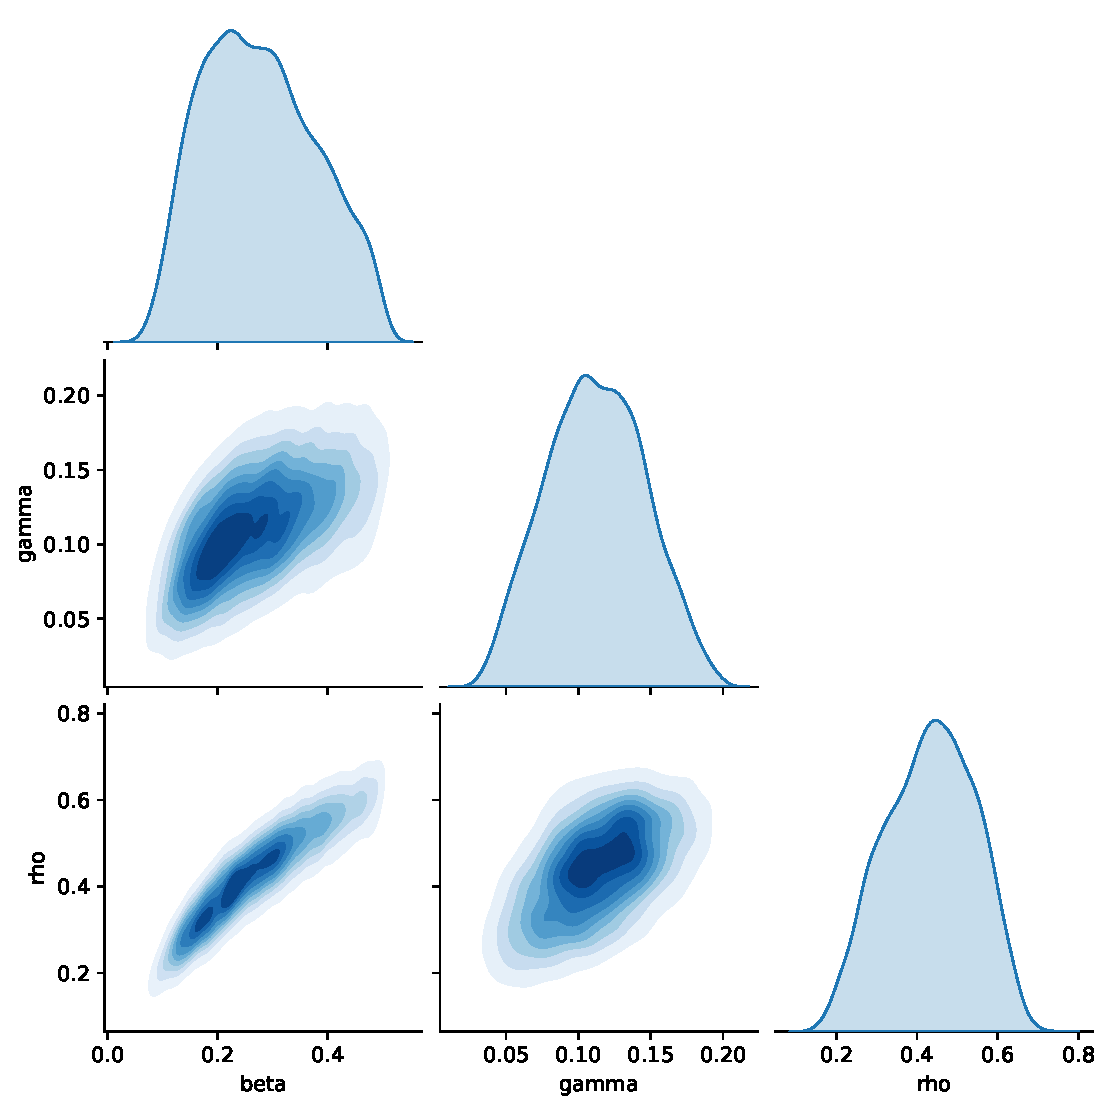
\includegraphics[width=0.6\textwidth]{plots/posterior_pairplot_s4_time.pdf}
    \caption{Pairwise posterior distributions obtained via Baseline ABC Rejection Sampling ($\epsilon=4.0$).}
    \label{fig:abc_rejection_pairplot}
\end{figure}

The resulting pairwise plots (Figure \ref{fig:abc_rejection_pairplot}) indicate that the posterior probability mass begins to localize within the parameter space, partially resolving the equifinality between $\beta$ and $\rho$.
However, the computational bottleneck caused by the curse of dimensionality restricted the number of accepted samples given a feasible time constraint \parencite{nott2014approximate}.
Consequently, the approximated posterior distribution remained relatively noisy and insufficiently dense for robust inference.
These results clearly demonstrate that naive rejection sampling is computationally inefficient for our parameter space, strongly motivating the transition to advanced sequential Monte Carlo methods.